\documentclass{article}

% Reference checking
% \usepackage{refcheck}

% Margins and page size
\usepackage[a4paper, margin=1in]{geometry}

% Babel
\usepackage[english]{babel}

% Smart quotes
\usepackage[autostyle, english = american]{csquotes}
\MakeOuterQuote{"}

% Package for matrices
\usepackage{amsmath}

% References
\usepackage{cite}

% Indent the first paragraph of each section
\usepackage{indentfirst}

% Set fonts
\usepackage{fontspec}
\setmainfont[Ligatures=TeX]{Times New Roman}
\setmonofont{Fira Code}[Scale=MatchLowercase]

% Figure captions
\usepackage{subcaption}
\usepackage[font=small,labelfont=bf]{caption}

% Image figures
\usepackage{graphicx}
\graphicspath{ {./img/} }

% Colors for code figures
\usepackage{color}
\definecolor{codegreen}{rgb}{0,0.6,0}
\definecolor{codegray}{rgb}{0.5,0.5,0.5}
\definecolor{codepurple}{rgb}{0.58,0,0.82}
\definecolor{backcolour}{rgb}{0.95,0.95,0.95}

% Define code figures
\usepackage{listings}
\lstdefinestyle{mystyle}{
    backgroundcolor=\color{backcolour},
    commentstyle=\color{codegreen},
    keywordstyle=\color{magenta},
    numberstyle=\small\color{codegray},
    stringstyle=\color{codepurple},
    basicstyle=\ttfamily,
    breakatwhitespace=false,
    breaklines=true,
    keepspaces=true,
    numbers=left,
    numbersep=5pt,
    showspaces=false,
    showstringspaces=false,
    showtabs=false,
    tabsize=2
}

% Use code format
\lstset{
    style=mystyle
}

% Set IEEE header and footer
\usepackage{fancyhdr}
\pagestyle{fancy}
\fancyhf{}
\renewcommand{\headrulewidth}{0pt}
\fancyfoot[R]{\thepage}

% Create title
\usepackage{titling}
\title{\Large\textbf{3D Graphics Rendering with OpenGL}}
\author{Jerred Shepherd}

% Document start
\begin{document}

% Title Page
\begin{titlingpage}
    \maketitle
    \begin{abstract}
    Computer graphics are an essential part to any consumer facing computer. Efficiently rendering computer graphics requires the use of specialized hardware in the form of graphics processing units. GPUs work differently compared to the CPUs which programmers are experienced with due to the former's focus on parallelization. Graphics APIs have been created to help programmers write performant and portable code for GPUs to render computer graphics. This paper will introduce the basic principles of 3D graphics rendering and OpenGL, a popular and widely-supported graphics API.
    \end{abstract}
\end{titlingpage}

% Body
\section{Introduction}
Computers have become widespread and have touched many aspects of modern-day life. From new forms of entertainment such as video games to artificial intelligence they have revolutionized the way to work, learn, and play. Computer graphics in particular have been a driving force behind the adoption of computers because they allow users to easily interact with computers. Programmers use computer graphics to display user interfaces, render video games, and even animate entire films. Every day millions of people interact with interfaces on phones, laptops, and other devices that allow them to focus on the work they are doing rather than how they communicate with their device. % TODO maybe this could still be improved

While there are plenty of tools to create and manipulate 2D and 3D graphics without writing graphics processing code, such as 3D object editors, image processing applications, UI libraries, and game engines, an understanding of the lower-level constructs allows a programmer to better use these higher-level abstractions and the opportunity to create their own when the existing tool do not meet their own unique use case. They can help a programmer to debug and optimize code since they will have an idea of how their higher-level usage is implemented down the stack.

This paper intends to introduce the reader to the broad concepts of graphics processing. This includes the purpose of graphics processing units, why graphics APIs exist, and an introduction to a commonly used cross-platform graphics API --- OpenGL. OpenGL will be discussed so that the reader has an overview of the concepts of OpenGL and can create an OpenGL program. This paper will focus on the use OpenGL version 3.2 which is widely supported and similar to newer versions of OpenGL.

\section{Background}
Graphics processing is predisposed towards parallel processing due to the repetitive and independent nature of calculations that it requires \cite[p.~4]{sellers2016}. Graphics processing units (GPUs) were created in order to meet the unique hardware requirements of computer graphics, and are fundamentally different from more traditional central processing units (CPUs). While CPUs generally have a few very fast cores, GPUs take an alternate approach of having a much greater number of slower cores. Figure \ref{fig:architecture} illustrates this difference in architecture, showing the massive difference in arithmetic logic units (ALUs) between CPUs and GPUs. These ALUs give GPUs an edge over CPUs when performing mathematical operations and are a core part of the parallel processing capability that GPUs posses.

\begin{figure}[h]
    \centering
    \begin{subfigure}[h]{0.39\textwidth}
    	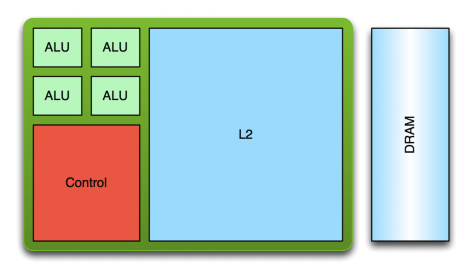
\includegraphics[width=\textwidth]{cpu}
    	\caption{CPU Architecture.}
    	\label{fig:cpu}
    \end{subfigure}
    \begin{subfigure}[h]{0.39\textwidth}
	    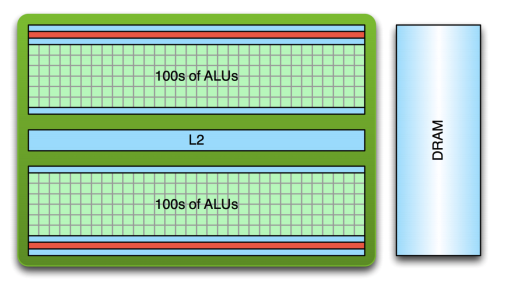
\includegraphics[width=\textwidth]{gpu}
	    \caption{GPU Architecture.}
	    \label{fig:gpu}
    \end{subfigure}
	\caption{A comparison of typical CPU and GPU architectures \cite{larkin2016}.}
	\label{fig:architecture}
\end{figure}

A difference also exists between the two in their approach of threading. An application running on a CPU may generally have only few threads running due to the high cost of creation and context switches. GPUs have lower cost thread creation and can more quickly context switch, and they often require tens of thousands of threads in order to fully reach their processing potential \cite{larkin2016}. Despite the slower performance of an individual GPU core GPUs easily outperform CPUs in tasks related to graphics processing due this difference in architecture which gives them an edge in parallel processing. Figure \ref{fig:performance} shows the historical theoretical performance gap between CPUs and GPUs in giga floating-point operations per second (GFLOP/s), a common measure of graphical computation speed. The graph shows that GPUs have clear performance advantage. Using GPUs effectively is especially important when rendering graphics since they often render items such as user interfaces which generally should remain responsive at all times.

\begin{figure}[h]
	\centering
	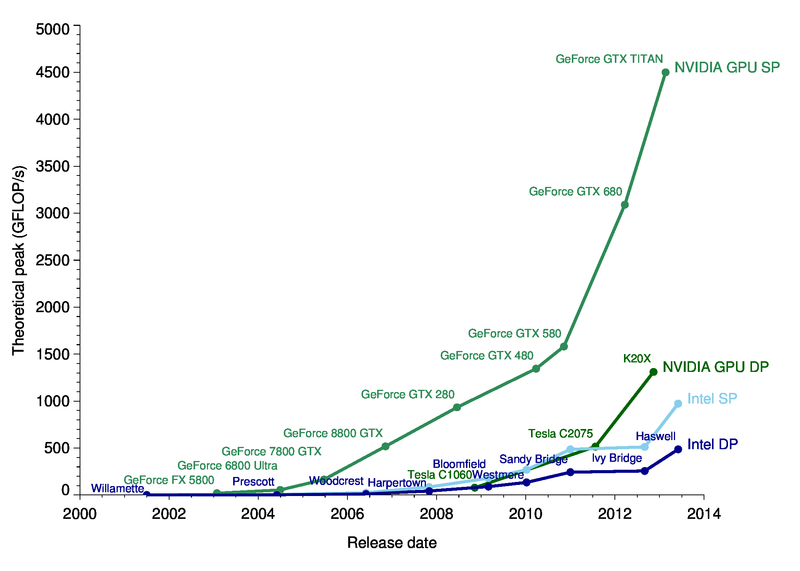
\includegraphics[height=7cm]{cpu-vs-gpu}
	\caption{A performance comparison of CPUs and GPUs in theoretical peak GLFOP/s over 14 years \cite{galloy2013}.}
	\label{fig:performance}
\end{figure}

Because of the architectural differences between GPUs and CPUs, GPUs are programmed differently than CPUs. In additional to writing high-level code which is compiled into assembly GPUs are also programmed by using APIs that are exposed by the manufacturer of the graphics card. GPU manufacturers may support proprietary APIs which is very common on cards that are made to be used in systems such as game consoles and arcade machines, or they may implement standardized APIs such as OpenGL, Metal, Vulkan, or DirectX.

While using a proprietary API may allow a programmer to get more performance out of the hardware they are targeting, it will severely limit the application's portability. A program that is written to run on a GPU using OpenGL should be compatible with any other GPU implementing the same version of OpenGL or higher. These APIs help programmers to focus on the code they are writing rather than what hardware it will be executed on and are created so that they are at a low enough level that maximum performance can be achieved while also being at a high enough level so that programmers can easily use them \cite[p.~4]{sellers2016}.

\section{Graphics Rendering}
Displays show images as a 2D matrix of pixels with the dimension of this matrix is referred to as its resolution. Traditionally each pixel of a color display has a red, blue, and green value which together determine the color of the pixel. Graphics rendering is how the color of these pixels are assigned to convey objects such as text, images, and user interfaces \cite{mckesson2018}. The higher the resolution of a display the more detail that can be shown on elements that are drawn. For reference displays commonly range from standard HD at 1280x720 to very high resolutions such as 3840 x 2160, referred to as 4K, which are becoming common on high-end monitors, TVs, and consumer electronics.

Graphics rendering is done by defining primitives such as points, lines, and triangles in a 3D space. After these points are defined their locations are transformed and they are drawn on the screen through a process called rasterization \cite{mckesson2018}. Figure \ref{fig:triangle-rendering} shows a simple example of the rasterization process. The figure begins by defining a triangle which is composed of three 3D vectors. The rasterizer then determines which pixels the triangle overlaps through a process called scan conversion. One way to do this is to include pixels if their centers are contained within the element. Rasterization then produces fragments, which is an element that contributes to the final color of a pixel \cite{sellers2016}. The fragments are assigned a color in later steps of the rendering process and which might be changed when effects such as lighting are taken into account.

Although these three primitives may seem simple and insignificant they are actually the backbone of graphics rendering. Complex 3D models such as those shown in video games are actually meshes of many small, connected triangles. Squares and other quadrilaterals can be created by connecting two triangles together at their hypotenuses.

\begin{figure}[h]
	\centering
	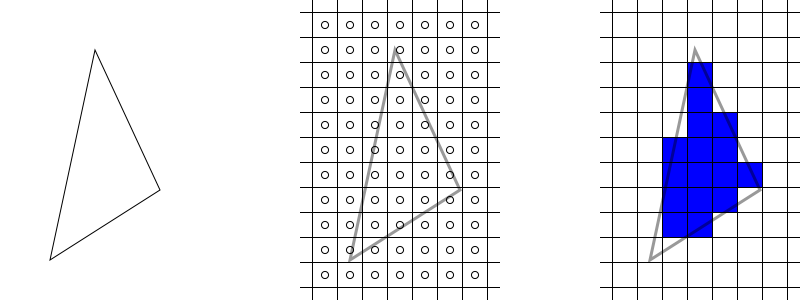
\includegraphics[height=3cm]{triangle-rendering}
	\caption{Rasterizing a triangle from three a triangle primitive \cite{mckesson2018}.}
	\label{fig:triangle-rendering}
\end{figure}

A two-dimensional object can easily be drawn by simply defining the x and y coordinates. Three-dimensional objects will not be drawn correctly at this point because the z coordinate does not affect the size of the object. The z coordinate represents how close a point is to a viewer with larger numbers being closer, therefore as the z coordinate increases the object should increase in size as well. This can be fixed by using a projection matrix and matrix multiplication. Each (x, y, z, w) coordinate will be multiplied by the matrix with the result being the location of the coordinate when projected onto the display. Before the matrix can be created the aspect ratio, field of view (fov), z-near, and z-far variables must first be determined. The aspect ratio is the ratio between a display's width and height, z-near and z-far represent the closest and furthest possible z coordinate values respectively, and fov is what angle that is visible on the screen. Figure \ref{fig:projection} shows an image illustration these four variables, and Figure \ref{fig:matrix} shows an example of a projection matrix used for 3D rendering. Orthogonal projection matrices also exist for 2D rendering however they are outside of the scope of this paper.

\begin{figure}[h]
	\centering
	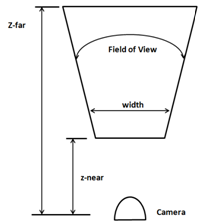
\includegraphics[height=4.5cm]{projection-matrix}
	\caption{Projection matrix concepts \cite{hernandez2019}.}
	\label{fig:projection}
\end{figure}

\begin{figure}[h]
    \[
	  \begin{bmatrix}
        \dfrac{\dfrac{1}{tan(\dfrac{f}{2})}}{a}  & 0 & 0 & 0 \\ \\
        0 & \dfrac{1}{tan(\dfrac{f}{2})} & 0 & 0 \\ \\
        0 & 0 & \dfrac{-(z_f + z_n)}{z_f - z_n} & \dfrac{-(2 * z_f * z_n)}{z_f - z_n} \\ \\
        0 & 0 & -1 & 0
      \end{bmatrix}
    \]
    \caption{A projection matrix where a is the aspect ratio, f is the field of view, $z_f$ is z-far, and $z_n$ is z-near \cite{hernandez2019}.}
    \label{fig:matrix}
\end{figure}

\section{OpenGL}
OpenGL is both a specification and a graphics API which is commonly implemented on modern graphics cards. The specification defines how the use of API should effect the graphics card. Like other graphics APIs, this allows users to use the underlying graphics hardware portably. OpenGL's development began at a computer hardware manufacturer named Silicon Graphics Inc. (SGI). SGI created its own proprietary graphics API named IrisGL which was used on its workstations and graphics hardware. IrisGL was cleaned up and in formalized into OpenGL. The first version of OpenGL released to the public as version 1.0 in 1992 \cite{openglwiki2018}. This initial version has been revised many times with the latest version being 4.6 which was released on July 31st, 2017 \cite{openglwiki2018}.

API bindings exist for C/C++ of which all other language bindings are based off of \cite{openglwiki2018}. Bindings exist for a wide variety of other languages such as python, C\#, and LISP and for every major operating system \cite{openglwiki2018}. The Lightweight Java Game Library (lwjgl) is a popular Java library that provides bindings for the OpenGL API and it will be used for example in this paper.

Before OpenGL can be used, an OpenGL context (i.e\. a desktop window) must be created. Many libraries exist to do this in a cross-platform manner. One popular library that is bundled with lwjgl is the Graphics Library Framework (GLFW) which makes it very easy to create an OpenGL context with lwjgl. Figure \ref{fig:glfw-creation} shows the code necessary to initialize the GLFW framework, create an operating system window with GLFW, and then finally bind an OpenGL context to it for drawing. Now that a window and OpenGL context have been created, OpenGL methods can be called and the window is ready to be drawn on.

\begin{figure}[h]
	\lstinputlisting[language=Java]{code/glfw.java}
	\caption{Creating a GLFW window and binding it to OpenGL in Java with lwjgl \cite{lwjgl}.}
	\label{fig:glfw-creation}
\end{figure}

\section{VBOs, VAOs, and Uniforms}
OpenGL provides the standard primitives used in graphics rendering --- points, lines, and triangles. All of these primitives are represented as float arrays which are passed to OpenGL for rendering. These float arrays are stored in vertex buffer objects (VBOs). VBOs are used to allocate memory on graphics hardware. Creating a VBO is simple however it would be beneficial to understand how the OpenGL APIs work before going into it.

The OpenGL API has state that is shared globally which includes what vertex array objects and vertex buffer objects are currently bound. Communication between the CPU and GPU is relatively slow so it should be minimized. Minimizing communication is done by buffering data to be drawn ahead of time and reusing the buffered data whenever possible. Due to the limitations of the JVM all memory being shared with native libraries must be allocated off of the JVM heap \cite{lwjglwiki}. lwjgl provides utilities to easily allocate this memory through the MemoryStack class. Data created on this stack can be sent to the graphics hardware with lwjgl. Unsigned integers, referred to as names, are used to uniquely identify OpenGL elements such as VBOs and VAOs. Many OpenGL functions take these names as arguments or rely on the currently bound VBO or VAO.

Figure \ref{fig:create-vbo} shows the code needed to store the vertices of a triangle on a graphics card. Line two asks OpenGL to create a new buffer name and store it. Next that buffer is bound so that all subsequent operations that require an array buffer will use it. An array of floats representing the vertices of a triangle are created, stored in native memory, and the finally transferred to the graphics card on line 22. VBO is now stored on the graphics card, but a VAO must first be created and bound before the VBO can be used.

\begin{figure}[h]
	\lstinputlisting[language=Java]{code/vbo.java}
	\caption{Creating a VBO and buffering vertex data with lwjgl.}
	\label{fig:create-vbo}
\end{figure}

A vertex array object stores state so that drawing can be done quickly and is required to be created before anything can be drawn. A VAO is bound and then setup so that when an object needs to be drawn in the future it only needs to be rebound without any further instruction before drawing. A vertex array simply keeps pointers to buffers which can and should be bound to multiple VAOs to save memory on the graphics hardware. Figure \ref{fig:vbo-vao-ebo} shows the relationship between vertex array objects and vertex buffer objects. Notice how the VAO has what is essentially an array of pointers to buffers. OpenGL allows you to set the pointer at each index to buffers that contain information about what is being drawn. Vertex buffer objects often contain vertex position coordinates, but they can contain other data used to render the element such as color and texture data.

\begin{figure}[h]
    \centering
	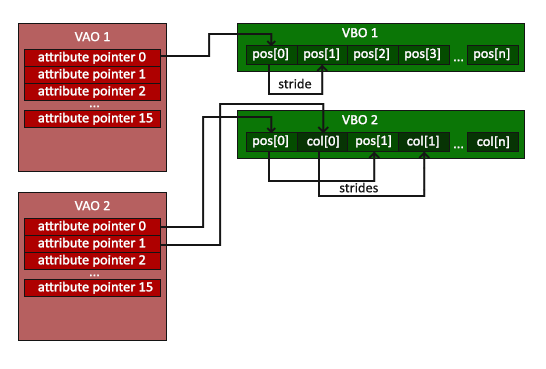
\includegraphics[height=6cm]{vao}
	\caption{Two VAOs with one VBO each \cite{devries2019}.}
	\label{fig:vbo-vao-ebo}
\end{figure}

As shown in Figure \ref{fig:create-vao}, creating a VAO is similar to creating a VBO. The glGenVertexArrays method allocates space for a VAO on the graphics card and returns its name. The name is then bound with the glBindVertexArray method so that all future methods that require a bound VAO use the newly created VAO. The previously created VBO is rebound on line 8 to ensure that the VAO points to the correct VBO. Line 11 sets the 0th index of the bound VAO to the currently bound VBO object. Its other arguments define the size, type, and layout of the data. The last step is to enable the 0th index on the VAO otherwise OpenGL will not pass the data when rendering.

\begin{figure}[h]
	\lstinputlisting[language=Java]{code/vao.java}
	\caption{Creating a VAO and binding a VBO to it.}
	\label{fig:create-vao}
\end{figure}

VAOs cannot bind more than 4 elements of a VBO array making it hard to pass large amounts of data to shaders while rendering. They also must be set per element which can be cumbersome if some data is shared between many elements. Uniforms are global variables which aim to solve this problem. Figure \ref{fig:matrix-uniform} shows a uniform being created to store a 4x4 projection matrix.

\begin{figure}[h]
	\lstinputlisting[language=Java]{code/uniform.java}
	\caption{Creating a 4x4 matrix uniform.}
	\label{fig:matrix-uniform}
\end{figure}

\section{The Rendering Pipeline}
Now that a VAO and VBO have been created OpenGL is almost ready to draw, the only thing left to do is to tell OpenGL what to do with the data it receives from VAOs, VBOs, and uniforms. When OpenGL receives a draw command, it runs the VAO through a pipeline before it is drawn on screen. This pipeline is responsible for repositioning, coloring, rasterizing, and applying effects such as lighting. The pipeline is divided into several stages many of which are configured through programs written in the OpenGL shading language (GLSL). Figure \ref{fig:pipeline-flow} shows a simplified view of the OpenGL pipeline and Figure \ref{fig:pipeline-visualized} shows how the input is transformed throughout the pipeline. Only two of these stages must have shaders written for them in order for rendering to occur which are the vertex and fragment shaders.

\begin{figure}[h]
    \centering
    \begin{subfigure}[h]{0.29\textwidth}
    	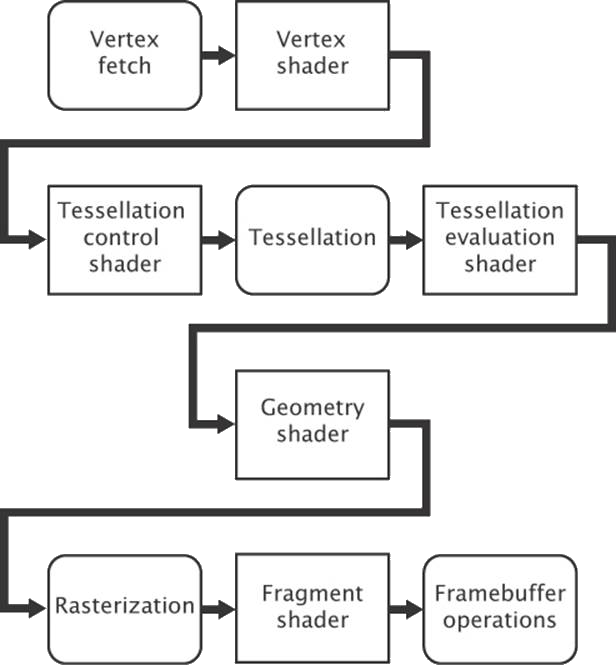
\includegraphics[width=\textwidth]{pipeline}
    	\caption{A simplified OpenGL pipeline \cite{sellers2016}.}
    	\label{fig:pipeline-flow}
    \end{subfigure}
    \begin{subfigure}[h]{0.49\textwidth}
	    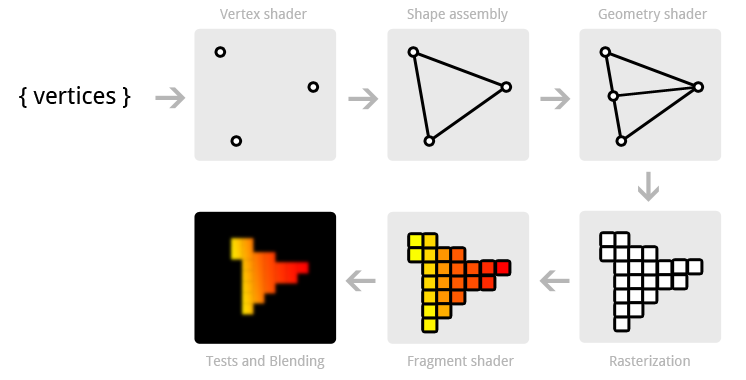
\includegraphics[width=\textwidth]{pipeline-visualized}
	    \caption{Visualization of data flowing through the OpenGL pipeline \cite{overvoorde2019}.}
	    \label{fig:pipeline-visualized}
    \end{subfigure}
	\caption{The OpenGL rendering pipeline.}
	\label{fig:pipeline}
\end{figure}

In order to customize the OpenGL pipeline a shader program must first be created. Once it is created, shaders can be compiled, attached to the program, and then linked. This final executable is run on the graphics hardware and executed by OpenGL when rendering. Figure \ref{fig:shader-program} shows the code needed to do create an OpenGL shader program.

\begin{figure}[b]
	\lstinputlisting[language=Java]{code/shaderProgram.java}
	\caption{Creating a shader program with a single shader.}
	\label{fig:shader-program}
\end{figure}

\subsection{Writing Shaders}

As mentioned before writing shaders is done in the OpenGL shading language which is based off of C. Figure \ref{fig:vertex-shader} shows a simple vertex shader program. The first line declares the version of OpenGL that the shader is using which is OpenGL 3.3 for this shader. Lines starting with "layout" tell OpenGL what input the shader is expecting. In this case this shader expects two inputs --- vectors of size 3 and size 4. The location indicates which index of the VAO these vectors should be found. The 0th index was set in Figure \ref{fig:create-vao} and represents the position of the element. The creation of the 1st index was omitted for brevity, however as the shader program shows it represents the color of the element. Lines starting with "out" indicate what data this shader passes on to future stages in the pipeline. Uniforms are global variables set. This shader contains only one uniform which is a 4x4 projection matrix.

The main function is where the work is being done. gl\_Position is a special variable that tells OpenGL the final position of an element. It is assigned to the input position after it is multiplied by the projection matrix. This position is passed on, as well as the color that was passed to the shader.

\begin{figure}[h]
	\lstinputlisting[language=C]{code/vertex.glsl}
	\caption{A simple vertex shader.}
	\label{fig:vertex-shader}
\end{figure}

The fragment shader partially determines the color of pixels. Figure \ref{fig:fragment-shader} shows a basic fragment shader which receives a color from the vertex shader in Figure \ref{fig:vertex-shader} and outputs the color as-is.

\begin{figure}[h]
	\lstinputlisting[language=C]{code/fragment.glsl}
	\caption{A simple fragment shader.}
	\label{fig:fragment-shader}
\end{figure}

Once all of this is put together, the application is ready to be compiled and a basic OpenGL program can be executed. This application will display a single triangle with its position and color specified by the code calling OpenGL. The output of the application can be seen in Figure \ref{fig:final-product}.

\begin{figure}[h]
    \centering
    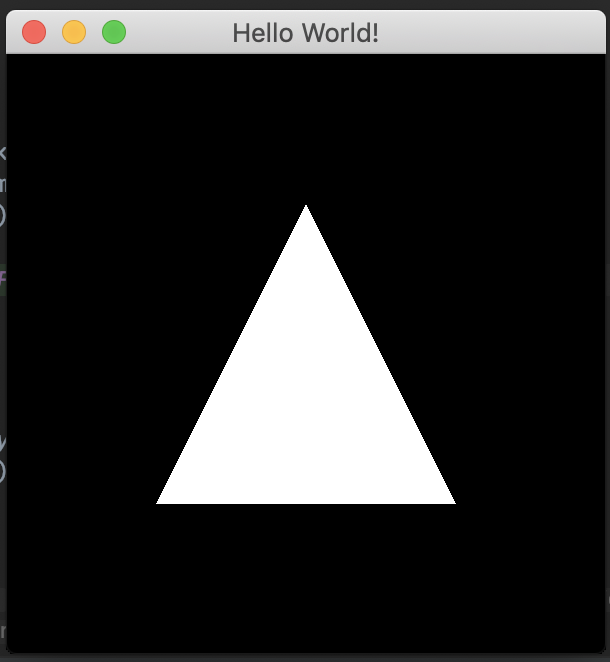
\includegraphics[height=6cm]{triangle}
	\caption{A triangle rendered from the vertices in Figure \ref{fig:create-vbo}.}
	\label{fig:final-product}
\end{figure}

\section{Conclusion}
Computer graphics are crucial to providing easy-to-use experiences for users and in creating modern day entertainment and other visual media. OpenGL allows you to render graphics by writing simple shader programs and feeding the OpenGL pipeline with input data. This data can then efficiently be rendered and displayed on screen to users. The pipeline can transform input and allows programmers to modify how their input is when rendering.

\clearpage

% References
\bibliography{bibliography}{}
\bibliographystyle{IEEEtran}

\end{document}